% ============================================================
%  SU2 Aeroacustica — Addendum Tecnico
%  DDES, Confronto FW-H vs APE, Implementazione APE in SU2
%  Aprile 2026 — Prof. A. Bottaro, Università di Genova
%  Committente: Huawei Research Finland
% ============================================================
\documentclass[11pt,a4paper]{article}

% ---------- encoding & lingua ----------
\usepackage[utf8]{inputenc}
\usepackage[T1]{fontenc}
\usepackage{lmodern}
\usepackage[italian]{babel}

% ---------- layout ----------
\usepackage[top=2.5cm,bottom=2.5cm,left=2.5cm,right=2.5cm]{geometry}
\usepackage[protrusion=true,expansion=false]{microtype}
\setlength{\headheight}{14pt}
\usepackage{parskip}
\setlength{\parskip}{0.5\baselineskip}
\setlength{\parindent}{0pt}

% ---------- matematica ----------
\usepackage{amsmath}
\usepackage{amssymb}
\usepackage{mathtools}

% ---------- grafica ----------
\usepackage{graphicx}
\graphicspath{{figs/}{figs_v2/}}
\usepackage{float}
\usepackage{caption}
\captionsetup{font=small,labelfont=bf,skip=6pt}
\usepackage{subcaption}

% ---------- tabelle ----------
\usepackage{booktabs}
\usepackage{tabularx}
\usepackage{array}
\usepackage{longtable}
\usepackage{multirow}

% ---------- colori ----------
\usepackage[table]{xcolor}
\definecolor{huaweiblue}{HTML}{1A365D}
\definecolor{midblue}{HTML}{2C5282}
\definecolor{lightblue}{HTML}{EBF4FF}
\definecolor{tablehead}{HTML}{D6E4F7}
\definecolor{codegray}{HTML}{444444}
\definecolor{codebg}{HTML}{F5F5F5}
\definecolor{keywordcolor}{HTML}{1A365D}
\definecolor{valuecolor}{HTML}{2C5282}
\definecolor{commentcolor}{HTML}{6A737D}

% ---------- listings ----------
\usepackage{listings}
\lstdefinestyle{SU2cfg}{%
  backgroundcolor=\color{codebg},
  basicstyle=\ttfamily\small,
  breaklines=true,
  breakatwhitespace=false,
  columns=fullflexible,
  keepspaces=true,
  frame=single,
  framerule=0.4pt,
  rulecolor=\color{midblue!40},
  tabsize=2,
  showstringspaces=false,
  commentstyle=\color{commentcolor}\itshape,
  morecomment=[l]{\%},
  keywordstyle=\color{keywordcolor}\bfseries,
  stringstyle=\color{valuecolor},
  morekeywords={SOLVER,KIND_TURB_MODEL,KIND_SGS_MODEL,MATH_PROBLEM,
    RESTART_SOL,INC_DENSITY_MODEL,INC_DENSITY_INIT,INC_VELOCITY_INIT,
    INC_NONDIM,VISCOSITY_MODEL,MU_CONSTANT,TIME_DOMAIN,TIME_MARCHING,
    TIME_STEP,MAX_TIME,INNER_ITER,CONV_RESIDUAL_MINVAL,NUM_METHOD_GRAD,
    CFL_NUMBER,MUSCL_FLOW,SLOPE_LIMITER_FLOW,CONV_NUM_METHOD_FLOW,
    TIME_DISCRE_FLOW,JST_SENSOR_COEFF,MARKER_INLET,MARKER_OUTLET,
    MARKER_HEATFLUX,ACOUSTIC_ANALOGY,MARKER_ACOUSTIC,OBSERVER_LOCATIONS,
    FREQ_LIMIT_FWH,OUTPUT_WRT_FREQ,VOLUME_OUTPUT,SCREEN_OUTPUT,
    HISTORY_OUTPUT,PARTITION_FILE,ITER,CFL_ADAPT,CFL_ADAPT_PARAM,
    CONV_NUM_METHOD_FLOW,HYBRID_RANSLES,WEIGHTED_LEAST_SQUARES,
    EULER_IMPLICIT,DUAL_TIME_STEPPING},
  literate={=}{{\textcolor{codegray}{=}}}1
}
\lstset{style=SU2cfg}

% ---------- hyperref ----------
\usepackage{hyperref}
\hypersetup{%
  colorlinks=true,
  linkcolor=huaweiblue,
  citecolor=midblue!70!black,
  urlcolor=midblue,
  pdftitle={SU2 Aeroacustica — Addendum: DDES, FW-H vs APE, implementazione APE},
  pdfauthor={Prof. A. Bottaro — Università di Genova},
  bookmarksnumbered=true
}

% ---------- section styling ----------
\usepackage{titlesec}
\titleformat{\section}{\large\bfseries\color{huaweiblue}}{\thesection}{1em}{}[\vspace{-4pt}\color{midblue}\rule{\linewidth}{0.4pt}\vspace{2pt}]
\titleformat{\subsection}{\normalsize\bfseries\color{midblue}}{\thesubsection}{1em}{}
\titleformat{\subsubsection}{\normalsize\bfseries\color{midblue!70!black}}{\thesubsubsection}{1em}{}

% ---------- comandi custom ----------
\newcommand{\ttcfg}[1]{\texttt{\color{codegray}#1}}
\newcommand{\kw}[1]{\texttt{\color{keywordcolor}\bfseries #1}}
\newcommand{\Djet}{D_{\mathrm{jet}}}
\newcommand{\Dcam}{D_{\mathrm{cam}}}
\newcommand{\Hcam}{H_{\mathrm{cam}}}
\newcommand{\Rey}{\mathrm{Re}}
\newcommand{\Ma}{\mathrm{Ma}}
\newcommand{\Str}{\mathrm{St}}
\newcommand{\mum}{\ensuremath{\,\mu\mathrm{m}}}
\newcommand{\mus}{\ensuremath{\,\mu\mathrm{s}}}
\providecommand{\ms}{}\renewcommand{\ms}{\ensuremath{\,\mathrm{ms}}}
\newcommand{\tFT}{t_{\mathrm{FT}}}

% ---------- header/footer ----------
\usepackage{fancyhdr}
\pagestyle{fancy}
\fancyhf{}
\fancyhead[L]{\small\color{midblue}\textit{Addendum Tecnico — SU2 Aeroacustica}}
\fancyhead[R]{\small\color{midblue}\textit{Huawei Research Finland / UniGe, Aprile 2026}}
\fancyfoot[C]{\small\thepage}
\renewcommand{\headrulewidth}{0.4pt}
\renewcommand{\headrule}{\color{midblue!40}\hrule width\headwidth height\headrulewidth}

% ============================================================
\begin{document}
% ============================================================

% -------- FRONTESPIZIO --------
\begin{titlepage}
  \centering
  \vspace*{1.5cm}

  {\color{huaweiblue}\rule{\linewidth}{1.5pt}}
  \vspace{0.6cm}

  {\huge\bfseries\color{huaweiblue}
    Addendum Tecnico:\\[0.4em]
    DDES, Confronto FW-H vs APE,\\[0.3em]
    Implementazione APE in SU2}

  \vspace{0.5cm}
  {\color{midblue}\rule{\linewidth}{0.6pt}}
  \vspace{0.8cm}

  {\large\itshape Supplemento al documento principale:\\
  \textit{``Simulazione SU2 Aeroacustica — Jet Impingente su Chip''}}

  \vspace{1.2cm}

  \begin{tabular}{rl}
    \textbf{Committente:} & Huawei Research Finland \\[4pt]
    \textbf{Referente UniGe:} & Prof.\ Alessandro Bottaro \\[4pt]
    \textbf{Dipartimento:} & DICCA — Università di Genova \\[4pt]
    \textbf{Data:} & Aprile 2026 \\[4pt]
    \textbf{Versione:} & 1.0 — Prima emissione \\
  \end{tabular}

  \vspace{1.5cm}
  {\color{huaweiblue}\rule{\linewidth}{1.5pt}}

  \vspace{1.0cm}
  {\normalsize
  \textbf{Oggetto del documento.} Questo addendum estende il paper principale
  su tre aspetti non trattati in dettaglio:
  \begin{enumerate}
    \item configurazione completa e criteri di accettazione per la simulazione DDES (Fase 4 della pipeline);
    \item analisi comparativa approfondita tra il metodo FW-H (Ffowcs-Williams Hawkings)
          e le equazioni APE (Acoustic Perturbation Equations);
    \item guida step-by-step all'integrazione di APE in SU2, che non dispone
          di tale solver nativamente.
  \end{enumerate}
  Il documento è destinato al gruppo di ricerca UniGe e agli ingegneri Huawei
  responsabili della valutazione acustica del sistema di raffreddamento a microjet.}

\end{titlepage}

% -------- SOMMARIO ESECUTIVO --------
\thispagestyle{fancy}
\section*{Sommario Esecutivo}
\addcontentsline{toc}{section}{Sommario Esecutivo}

Il paper principale descrive una pipeline di simulazione in cinque fasi
(mesh, RANS, URANS, DDES/LES, post-processing acustico) per la caratterizzazione
del rumore prodotto da un jet impingente su chip in una camera di raffreddamento
con geometria D\,=\,20\,mm $\times$ H\,=\,3\,mm.
Il committente Huawei Research Finland ha richiesto tre approfondimenti specifici
che motivano la redazione del presente addendum.

\textbf{Obiettivo 1 — DDES operativo (Sezione~\ref{sec:ddes}).}
La Fase 4 della pipeline prevede una simulazione DDES Spalart-Allmaras come
strategia ibrida RANS/LES economicamente accessibile su HPC di livello dipartimentale.
Il paper principale accenna ai parametri senza fornire il setup completo.
Questo addendum documenta ogni opzione del file di configurazione SU2,
i criteri di accettazione fisici (pendenza $-5/3$, funzione di protezione
$f_d \geq 0.95$, assenza di Modeled-Stress Depletion), e il piano di monitoraggio
runtime.

\textbf{Obiettivo 2 — Scelta del metodo acustico (Sezioni~\ref{sec:teoria}--\ref{sec:raccomandazione}).}
Il metodo FW-H, nativo in SU2, è lo standard per il post-processing acustico
in jet liberi. Tuttavia la geometria confinata del caso Huawei e la prospettiva
futura di introdurre una mesh cubica (barriera fonoassorbente) pongono interrogativi
sulla sua adeguatezza. L'addendum sviluppa un confronto rigoroso con il metodo APE,
analizza le limitazioni di ciascun approccio in relazione alla geometria specifica,
e formula una raccomandazione per la commessa corrente e quella successiva.

\textbf{Obiettivo 3 — Roadmap implementativa APE (Sezioni~\ref{sec:ape}--\ref{sec:implementazione}).}
APE non è disponibile in SU2. L'addendum identifica e valuta tre opzioni di
integrazione (coupling con libAcoustics/OpenFOAM, solver custom Python/C++,
fork SU2 con nuova classe solver), con stima di tempi, rischi e costi per
ciascuna.

\medskip
\textbf{Conclusione anticipata.} Per la commessa attuale FW-H è adeguato;
per Fase 2 (mesh cubica) sarà necessario APE, con Opzione A
(coupling libAcoustics) raccomandata per il rapporto rischio/costo.

\clearpage

% -------- INDICE --------
\tableofcontents
\clearpage

% ============================================================
\section{Configurazione Dettagliata DDES — Fase 4 della Pipeline}
\label{sec:ddes}
% ============================================================

\subsection{Fondamenti del modello SA-DDES}

La simulazione Delayed Detached-Eddy Simulation (DDES) nella variante
Spalart-Allmaras \cite{spalart2006} è il compromesso computazionale adottato
nella Fase 4 della pipeline. Il modello opera come RANS ($k$-$\varepsilon$ di
Spalart-Allmaras) all'interno del boundary layer e commuta verso un comportamento
LES (via riduzione della viscosità di sgomberato) nelle regioni di shear layer
e scia dove le strutture turbolente energetiche sono fattivamente risolvibili
dalla mesh.

La transizione è governata dalla funzione di protezione $f_d$, definita come:
\[
  f_d = 1 - \tanh\!\left[(8\,r_d)^3\right],
  \qquad
  r_d = \frac{\tilde{\nu}}{\sqrt{U_{i,j}\,U_{i,j}}\,\kappa^2 d^2}
\]
dove $\tilde{\nu}$ è la viscosità cinematica modificata del modello SA, $U_{i,j}$
il tensore gradiente di velocità, $\kappa = 0.41$ la costante di von Kármán,
e $d$ la distanza dalla parete.
Quando $f_d \approx 0$ (strato limite) il modello agisce come RANS pieno;
quando $f_d \approx 1$ (bulk/shear layer) si attiva il ramo LES.

La lunghezza di scala modificata che pilota la transizione è:
\[
  \tilde{d} = d - f_d \cdot \max\!\bigl(0,\; d - C_\mathrm{DES}\,\Delta\bigr)
\]
dove $C_\mathrm{DES} = 0.65$ (valore di default in SU2 v8) e
$\Delta = \max(\Delta x, \Delta y, \Delta z)$ è la dimensione massima
della cella locale. Il prefisso ``Delayed'' rispetto all'originale DES97
indica proprio la protezione aggiuntiva via $f_d$ per evitare la ``gray area''
RANS$\to$LES in prossimità della parete.

\subsection{Parametri numerici raccomandati}

I seguenti parametri sono ottimizzati per la mesh L3 ($\approx 3 \times 10^6$
celle, $\Delta x_\mathrm{min} = 30\mum$) sul caso Huawei:

\begin{table}[H]
  \centering
  \caption{Parametri numerici raccomandati per la simulazione DDES — Mesh L3.}
  \label{tab:ddes_params}
  \begin{tabular}{lll}
    \toprule
    \textbf{Parametro} & \textbf{Valore} & \textbf{Motivazione} \\
    \midrule
    $\Delta t$ & $5 \times 10^{-6}$\,s & CFL $\leq 1$ su $\Delta x_\mathrm{min}=30\mum$, $U_\mathrm{jet}=10$\,m/s \\
    Durata simulazione & 40\ms\ = $10\,\tFT$ & Convergenza statistica spettrali \\
    Preflush (da scartare) & 10\ms\ = $2.5\,\tFT$ & Lavaggio transitori iniziali \\
    Step fisici totali & 8\,000 & $40\ms / 5\mus$ \\
    \kw{INNER\_ITER} & 25 & Sufficiente per residuo $-5$ in dual time \\
    \kw{CONV\_RESIDUAL\_MINVAL} & $-5$ & Meno stringente di LES (economica) \\
    \kw{SLOPE\_LIMITER\_FLOW} & \texttt{NONE} & Nessuna dissipazione artificiale in zona LES \\
    \kw{CONV\_NUM\_METHOD\_FLOW} & \texttt{ROE} & Upwind limitato, stabile \\
    \kw{MUSCL\_FLOW} & \texttt{YES} & Ricostruzione 2° ordine spaziale \\
    \kw{TIME\_DISCRE\_FLOW} & \texttt{EULER\_IMPLICIT} & Stabilità per dual time stepping \\
    \bottomrule
  \end{tabular}
\end{table}

\subsection{File di configurazione SU2 annotato}

Il listing seguente riporta il file \texttt{ddes\_sa.cfg} con ogni opzione
commentata per chiarire la motivazione fisica o numerica della scelta.

\begin{lstlisting}[style=SU2cfg, caption={File di configurazione SU2 v8 per DDES SA — Fase 4 della pipeline. Commenti riga per riga.}, label=lst:ddes_cfg]
% ============================================================
%  SU2 v8 — DDES Spalart-Allmaras (fase 4 pipeline)
%  Mesh L3 (~3M celle), HPC preferito (laptop borderline)
%  Obiettivo: verifica pendenza -5/3 nello shear layer
% ============================================================

% --- Tipo di solver e modello turbolento ---
SOLVER= INC_RANS          % Solver incompressibile (Ma=0.029 << 0.3)
KIND_TURB_MODEL= SA       % Spalart-Allmaras: modello base DDES
HYBRID_RANSLES= SA_DDES   % Attiva la variante DDES con f_d di protezione
MATH_PROBLEM= DIRECT      % Forward problem (non aggiunto, non ottimizzazione)
RESTART_SOL= YES          % Ripartire dalla soluzione URANS convergente (Fase 3)

% --- Proprietà del fluido (aria, T=293 K, p_atm) ---
INC_DENSITY_MODEL= CONSTANT    % Densita' costante (incompressibile)
INC_DENSITY_INIT= 1.225        % kg/m^3 a 293 K, 1 atm
INC_VELOCITY_INIT= (0.0, 0.0, -10.0)  % m/s: jet nella direzione -z
VISCOSITY_MODEL= CONSTANT_VISCOSITY
MU_CONSTANT= 1.8375E-5         % Pa*s a 293 K (Sutherland evalutato a T_ref)

% --- Integrazione temporale ---
TIME_DOMAIN= YES
TIME_MARCHING= DUAL_TIME_STEPPING-2ND_ORDER  % Schema BDF2, accurato in tempo
TIME_STEP= 5.0E-6    % Delta_t = 5 us -> CFL ~ 1 su Delta_x_min = 30 um
MAX_TIME= 0.040      % 40 ms = 10 tempi di flush (t_FT ~ 4 ms per L=20mm, U=5 m/s)
INNER_ITER= 25       % Iterazioni interne per dual time: bilancio costo/convergenza
CONV_RESIDUAL_MINVAL= -5  % Sufficiente per DDES; LES userebbe -6 o -7

% --- Schema numerico di flusso ---
CFL_NUMBER= 15.0            % CFL per il time step fisico (non le inner iterations)
NUM_METHOD_GRAD= WEIGHTED_LEAST_SQUARES  % Gradiente WLS: robusto su mesh ibrida
MUSCL_FLOW= YES             % Ricostruzione MUSCL di 2° ordine
SLOPE_LIMITER_FLOW= NONE    % NO limiter: evita dissipazione artificiale nella zona LES
CONV_NUM_METHOD_FLOW= ROE   % Schema di Roe: upwind, stabile, 2° ordine con MUSCL
TIME_DISCRE_FLOW= EULER_IMPLICIT  % Integrazione implicita delle inner iterations

% --- Condizioni al contorno ---
MARKER_INLET= ( jet_inlet, 293.15, 10.0, 0.0, 0.0, -1.0 )
% (marker, T_total[K], v_mag[m/s], nx, ny, nz)
MARKER_OUTLET= ( lateral_outlet, 0.0 )
% Pressione manometrica nulla all'outlet laterale della camera
MARKER_HEATFLUX= ( chip_wall, 0.0 )    % Parete adiabatica: chip (bottom)
MARKER_HEATFLUX= ( top_plate, 0.0 )    % Parete adiabatica: coperchio (top)
MARKER_HEATFLUX= ( inlet_tube_wall, 0.0 ) % Parete adiabatica: tubo di ingresso

% --- Output ---
OUTPUT_WRT_FREQ= 200  % Scrittura ogni 200 step = 1 ms: ~200 snapshot per spettro
VOLUME_OUTPUT= COORDINATES, SOLUTION, PRIMITIVE, VORTICITY, Q_CRITERION
% F_D (funzione protezione DDES) e EDDY_VISCOSITY devono essere aggiunti
% se la versione SU2 in uso li espone come campi di volume separati.
% Verificare con: grep -r "F_D" $SU2_HOME/SU2_CFD/src/output
SCREEN_OUTPUT= (INNER_ITER, RMS_PRESSURE, RMS_VELOCITY-X, LINSOL_RESIDUAL)
HISTORY_OUTPUT= ITER, RMS_RES, AERO_COEFF
\end{lstlisting}

\subsection{Campi di volume per il monitoraggio runtime}

I campi raccomandati in \kw{VOLUME\_OUTPUT} per la diagnostica DDES sono:

\begin{itemize}
  \item \texttt{F\_D}: funzione di blending. Deve essere $\geq 0.95$ in almeno
        l'80\% del volume dello shear layer per confermare che la simulazione
        opera effettivamente come LES in quella regione.
  \item \texttt{EDDY\_VISCOSITY}: viscosità turbolenta $\mu_t$. Nella zona LES
        $\mu_t$ deve ridursi a valori paragonabili a $\mu$ molecolare; valori
        elevati indicano che il modello RANS non si è ``spento''.
  \item \texttt{VORTICITY}: campo di vorticità $|\boldsymbol{\omega}|$;
        utile per visualizzare le strutture coerenti nello shear layer.
  \item \texttt{Q\_CRITERION}: secondo invariante del tensore gradiente di
        velocità, usato per l'isosuperficie delle strutture turbolente.
\end{itemize}

Con \kw{OUTPUT\_WRT\_FREQ}\,=\,200 e $\Delta t = 5\mus$ si ottengono 200
snapshot al secondo fisico (200 file da $\approx$50\,MB ciascuno su mesh L3
con campi full double precision), per un totale atteso di $\approx$6\,GB
per la sola fase DDES.

\subsection{Criteri di accettazione fisici}

Prima di procedere al post-processing acustico, verificare:

\begin{enumerate}
  \item \textbf{Attivazione LES effettiva:} $f_d \geq 0.95$ in almeno l'80\%
        del volume della shear layer (regione $r > D_\mathrm{jet}/2$,
        $0 < z < H_\mathrm{cam}$). Se il criterio non è soddisfatto la mesh
        è troppo grossolana: raffinare a L4 o ridurre $C_\mathrm{DES}$
        a 0.55.
  \item \textbf{Pendenza spettrale $-5/3$:} lo spettro di energia cinetica
        turbolenta $E(k)$ estratto nella shear layer deve mostrare il range
        inerziale di Kolmogorov ($\sim k^{-5/3}$) su almeno mezza decade in
        numero d'onda. Questa condizione garantisce che le strutture energetiche
        siano risolte e non smorzate dalla viscosità numerica.
  \item \textbf{Assenza di Modeled-Stress Depletion (MSD):} la ``gray area''
        RANS$\to$LES non deve presentare una transizione allargata (>5\% di
        $L_\mathrm{cam}$). In presenza di MSD considerare il passaggio a
        IDDES (\kw{HYBRID\_RANSLES}\,=\,\texttt{SA\_IDDES}).
  \item \textbf{Convergenza statistica:} i momenti del secondo ordine
        ($\langle u'u' \rangle$, $\langle p'p' \rangle$) devono stabilizzarsi
        entro $\pm 2\%$ tra la prima e la seconda metà della finestra temporale
        utile (20\ms).
\end{enumerate}

\subsection{Script di post-processing per la verifica diagnostica}

Il seguente pseudocodice Python illustra la verifica dei criteri 1 e 3:

\begin{lstlisting}[language=Python, style=SU2cfg,
  caption={Pseudocodice Python per la verifica di $f_d$ e MSD nel volume di output DDES.},
  label=lst:ddes_postproc]
import pyvista as pv
import numpy as np

# Carica un volume output SU2 (formato VTK/CGNS)
mesh = pv.read("volume_00200.vtu")

# Estrai F_D e coordinate
fd = mesh["F_D"]
xyz = mesh.points
z   = xyz[:, 2]
r   = np.sqrt(xyz[:, 0]**2 + xyz[:, 1]**2)

# Definisci shear layer: r > D_jet/2, 0 < z < H_cam
D_jet = 2e-3      # m
H_cam = 3e-3      # m
mask_sl = (r > D_jet/2) & (z > 0) & (z < H_cam)

# Criterio 1: f_d >= 0.95 in almeno 80% dello shear layer
frac_les = np.mean(fd[mask_sl] >= 0.95)
print(f"Frazione LES nello shear layer: {frac_les:.1%}")
if frac_les < 0.80:
    print("AVVISO: attivazione LES insufficiente. Raffinare mesh o ridurre C_DES.")

# Criterio 3: larghezza gray area
# Sull'asse di simmetria (r < 0.5*D_jet), trova la transizione f_d 0.1 -> 0.9
mask_axis = r < D_jet / 2
z_axis = z[mask_axis]
fd_axis = fd[mask_axis]
idx_sort = np.argsort(z_axis)
z_s = z_axis[idx_sort]
fd_s = fd_axis[idx_sort]
z_10 = z_s[np.searchsorted(fd_s, 0.10)]
z_90 = z_s[np.searchsorted(fd_s, 0.90)]
gray_area_width = abs(z_90 - z_10)
print(f"Larghezza gray area: {gray_area_width*1e3:.2f} mm")
if gray_area_width > 0.05 * 20e-3:
    print("AVVISO: gray area estesa. Valutare IDDES.")
\end{lstlisting}

% ============================================================
\section{Teoria del Problema Acustico in Dominio Confinato}
\label{sec:teoria}
% ============================================================

\subsection{Separazione di scale}

Nel caso Huawei il numero di Mach del jet è $\Ma \approx 0.029$
($U_\mathrm{jet} = 10$\,m/s, $c_0 = 343$\,m/s a 293\,K), che colloca il
flusso nel regime aeroacustico basso-Mach.
A basso Mach la separazione tra scala idrodinamica e scala acustica è netta:
la lunghezza d'onda acustica minima di interesse (20\,kHz) è
\[
  \lambda_{\min} = \frac{c_0}{f_{\max}} = \frac{343}{20\,000} \approx 17.15\,\mathrm{mm},
\]
molto maggiore delle strutture turbolente energetiche
($\ell_\mathrm{hydro} \sim D_\mathrm{jet}/2 = 1$\,mm).
Il campo prossimale è quindi quasi incompressibile e il campo acustico è
una perturbazione di ampiezza $O(\Ma^2)$ sovrapposta ad esso.

\subsection{Effetti specifici del confinamento}

La geometria confinata
($\Dcam = 20$\,mm, $\Hcam = 3$\,mm) introduce fenomeni assenti nei getti liberi:

\paragraph{Modi acustici della cavità.}
Le frequenze proprie della cavità rettangolare (approssimata) sono
$f_{n,m} = (c_0 / 2)\sqrt{(n/L_x)^2 + (m/L_z)^2}$.
Per la dimensione verticale $L_z = 3$\,mm:
\[
  f_{1,0}^{(z)} = \frac{c_0}{2 L_z} = \frac{343}{2 \times 3 \times 10^{-3}} \approx 57\,\mathrm{kHz}
\]
che supera la banda di analisi. Per la dimensione radiale $L_x = D_\mathrm{cam}/2 = 10$\,mm:
\[
  f_{1,0}^{(r)} \approx \frac{c_0}{2 L_x} = \frac{343}{2 \times 10^{-2}} \approx 17.15\,\mathrm{kHz}
\]
nella banda di interesse. Questo modo può generare picchi di risonanza
che FW-H in spazio libero non è in grado di predire correttamente.

\paragraph{Riflessioni da pareti no-slip.}
Le pareti superiore (top plate) e inferiore (chip) riflettono le onde acustiche.
In una camera con $\Hcam \ll \lambda_{\min}$ (3\,mm $\ll$ 17\,mm a 20\,kHz) il
confinamento verticale impone un campo quasi-bidimensionale nelle onde a bassa
frequenza, alterando la direttività rispetto al caso libero.

\paragraph{Trade-off nella scelta della superficie FW-H.}
Una superficie FW-H permeabile troppo vicina alla sorgente cattura fluttuazioni
di pressione idrodinamica (``pseudo-suoni'') non propaganti, che contaminano
lo spettro. Una superficie troppo distante — vicina alle pareti — è immersa nel
campo riflesso, che FW-H interpreta come sorgente reale.

\subsection{Scale temporali e banda di analisi}

La finestra temporale utile (20\ms) e il passo temporale $\Delta t = 5\mus$ danno:
\begin{itemize}
  \item risoluzione in frequenza: $\Delta f = 1/(20\,\mathrm{ms}) = 50$\,Hz;
  \item frequenza di Nyquist: $f_N = 1/(2\Delta t) = 100$\,kHz;
  \item banda target: 0.5–20\,kHz (compatibile con il microfono MEMs Huawei).
\end{itemize}

\subsection{Panoramica degli approcci acustici}

Tre classi di metodi sono applicabili al caso in esame:

\begin{enumerate}
  \item \textbf{Analogia integrale (FW-H, Curle):} post-processing su superficie
        di controllo, Green's function in spazio libero. Implementato nativamente
        in SU2.
  \item \textbf{Equazioni linearizzate (APE, LEE):} solver PDE aggiuntivo per
        le perturbazioni acustiche, con sorgenti estratte dal CFD. Non presente
        in SU2. Cattura rifrazione, diffrazione, riflessioni.
  \item \textbf{DNS compressibile diretto:} il campo acustico è risolto nella
        stessa simulazione CFD. Impraticabile per geometrie industriali a basso
        Mach (la risoluzione richiesta per il campo acustico è $O(10^3 \times)$
        più grossolana di quella per la turbolenza, ma vanno risolte entrambe).
\end{enumerate}

Nei capitoli seguenti sono sviluppati i metodi 1 e 2.

% ============================================================
\section{Metodo FW-H (Ffowcs-Williams Hawkings)}
\label{sec:fwh}
% ============================================================

\subsection{Derivazione sintetica}

L'equazione di Ffowcs-Williams e Hawkings \cite{fwh1969} è un'equazione d'onda
non omogenea che generalizza l'analogia di Lighthill alla presenza di superfici
solide in moto arbitrario:
\[
  \Box^2 p' = \frac{\partial^2 T_{ij}}{\partial x_i \partial x_j}
  - \frac{\partial}{\partial x_i}\bigl[F_i\,\delta(f)\bigr]
  + \frac{\partial}{\partial t}\bigl[Q\,\delta(f)\bigr]
\]
dove $\Box^2 = \partial^2/\partial t^2 - c_0^2\,\nabla^2$, $T_{ij}$ è il
tensore di Lighthill, $F_i$ il termine dipolaro di superficie (forze) e
$Q$ il termine monopolare (spostamento di massa).
L'integrazione formale via Green's function in spazio libero fornisce la
pressione acustica $p'(\mathbf{x},t)$ in un osservatore remoto come integrale
sulla superficie di controllo $f=0$.

\subsection{Formulazione Farassat 1A}

SU2 implementa la formulazione Farassat 1A \cite{farassat2007}, che esprime
$p'$ in dominio temporale come:
\[
  4\pi\,p'(\mathbf{x},t) = \int_f \left[\frac{\dot{L}_r}{r(1-M_r)^2}\right]_\tau \mathrm{d}S
  + \int_f \left[\frac{L_r\bigl(r\dot{M}_r + c_0(M_r - M^2)\bigr)}{r^2(1-M_r)^3}\right]_\tau \mathrm{d}S
\]
dove $L_r$ è la componente radiale del carico di superficie, $M_r$ il numero
di Mach nella direzione dell'osservatore, e $[\cdot]_\tau$ indica la valutazione
al tempo ritardato $\tau$.

\subsection{Superficie FW-H: solida vs permeabile}

\begin{description}
  \item[Superficie solida (corpo reale):] include solo i termini monopolari
        e dipolari sulla parete del solido. Cattura il rumore da carico
        (dipolare) ma perde i quadrupoli volumetrici nella zona di mescolamento
        del jet, rilevanti già a $\Ma > 0.1$.
  \item[Superficie permeabile (virtual surface):] racchiude il volume sorgente
        e include tutti i contributi (monopoli + dipoli + quadrupoli) entro
        la superficie. È il metodo raccomandato per jet ad alto contenuto
        turbolento.
\end{description}

\subsection{End-cap correction}

Per configurazioni con flusso in ingresso/uscita attraverso la superficie
FW-H (throughflow), i pannelli terminali (end-caps) generano contributi
spuri dovuti alla presenza di fluttuazioni idrodinamiche non propaganti.
La correzione di Shur e Spalart \cite{shur2005} sopprime tali contributi
applicando una finestra spaziale sui pannelli terminali.
Si raccomanda di verificarne l'attivazione per il caso Huawei, dove la
superficie permeabile è attraversata da flusso nella direzione verticale.

\subsection{Implementazione in SU2}

Le opzioni rilevanti del file di configurazione SU2 sono:

\begin{lstlisting}[style=SU2cfg, caption={Opzioni SU2 per l'analisi acustica FW-H.}, label=lst:fwh_cfg]
% --- Analogia acustica FW-H ---
ACOUSTIC_ANALOGY= FWH
% Seleziona il metodo di Ffowcs-Williams Hawkings (alternativa: CURLE)

MARKER_ACOUSTIC= ( fwh_surface )
% Nome del marker che definisce la superficie FW-H permeabile nel file mesh.
% La superficie deve essere chiusa (volume sorgente completamente racchiuso).

OBSERVER_LOCATIONS= fwh_observers.dat
% File testo con le coordinate (x,y,z) degli osservatori acustici.
% Formato: una terna per riga, in metri.

FREQ_LIMIT_FWH= 25000
% Frequenza di Nyquist FW-H in Hz. Valore conservativo: usa l'effettivo
% Nyquist del timestep (100 kHz) filtrato a 25 kHz per ridurre lo spettro.
\end{lstlisting}

\subsection{Costo computazionale}

Il costo di FW-H è $O(N_\mathrm{obs} \times N_\mathrm{steps} \times N_\mathrm{panels})$,
tipicamente 5–15\% del costo totale della simulazione LES.
Il calcolo è eseguito in post-processing (nessuna PDE aggiuntiva online).

\subsection{Pro e contro del metodo FW-H}

\textbf{Punti di forza:}
\begin{itemize}
  \item Post-processing only: nessun solver PDE aggiuntivo da risolvere durante
        la simulazione.
  \item Nativamente implementato e validato in SU2 con test benchmark di
        riferimento (getto cilindrico BANC-I).
  \item Compatibile con qualunque campo CFD incompressibile o compressibile
        senza modifiche al solver principale.
  \item Ideale per jet liberi e geometrie aperte senza ostacoli tra sorgente
        e osservatore.
\end{itemize}

\textbf{Limitazioni:}
\begin{itemize}
  \item La Green's function utilizzata è quella dello spazio libero: il metodo
        non cattura riflessioni, diffrazioni né rifrazioni dovute a ostacoli
        o pareti esterne alla superficie di controllo.
  \item Assume propagazione in mezzo omogeneo quiescente o con flusso medio
        uniforme: le variazioni di velocità media (gradienti di taglio forti)
        che inducono rifrazione non sono modellate.
  \item In dominio confinato con pareti riflettenti (come la camera Huawei)
        l'accuratezza si riduce per $f > f_\mathrm{risonanza}$
        (circa 8–17\,kHz nel caso in esame).
  \item Non adatto se sono presenti ostacoli solidi tra sorgente e osservatore
        (es.\ mesh cubica fonoassorbente prevista in Fase 2).
\end{itemize}

% ============================================================
\section{Metodo APE (Acoustic Perturbation Equations)}
\label{sec:ape}
% ============================================================

\subsection{Idea fondamentale e riferimento seminale}

Le Acoustic Perturbation Equations sono state introdotte da Ewert e
Schröder \cite{ewert2003} con l'obiettivo di separare formalmente il campo
idrodinamico (vorticità, campi di pressione pseudo-sonora) dal campo acustico
(onde propaganti), e di scrivere equazioni di evoluzione PDE stabili per
la sola componente acustica.

La decomposizione parte da:
\[
  \mathbf{u} = \mathbf{\bar{u}} + \mathbf{u}_h + \mathbf{u}', \qquad
  p = \bar{p} + p_h + p'
\]
dove il soprascritto $\bar{(\cdot)}$ denota la media temporale RANS,
il pedice $h$ il contributo idrodinamico non stazionario (estratto dal CFD),
e l'apice $'$ la perturbazione acustica.
Il campo sorgente è fornito dal simulatore CFD (LES/DDES) in modo disaccoppiato
(\textit{one-way coupling}): CFD $\to$ APE.

\subsection{Formulazione APE-2}

La variante APE-2, adottata per flussi aeroacustici a basso Mach, è:
\begin{align}
  \frac{\partial p'}{\partial t} + c_0^2 \nabla \cdot \bigl(\rho_0 \mathbf{u}'\bigr)
    &= -\frac{\partial p'_e}{\partial t} \label{eq:ape2_p} \\[6pt]
  \frac{\partial \mathbf{u}'}{\partial t} + \nabla\bigl(\mathbf{\bar{u}} \cdot \mathbf{u}'\bigr)
    + \nabla\!\left(\frac{p'}{\rho_0}\right)
    &= \mathbf{q}_m \label{eq:ape2_u}
\end{align}
dove:
\begin{itemize}
  \item $p'_e = p - \bar{p} - p_h$ è la pressione di eccitazione acustica
        (differenza tra pressione totale istantanea CFD e componenti non acustiche);
  \item $\mathbf{q}_m = -\boldsymbol{\omega}_h \times \mathbf{\bar{u}}$
        è il termine sorgente di Lamb (vorticità idrodinamica $\times$ velocità media),
        principale generatore di rumore aerodinamico;
  \item $c_0$, $\rho_0$ sono costanti del mezzo a riposo (o funzioni lentamente
        variabili se il background non è omogeneo).
\end{itemize}

\subsection{Proprietà di stabilità}

La proprietà più rilevante di APE rispetto alle Linearized Euler Equations
(LEE) è la stabilità algebrica: le APE non supportano le instabilità
idrodinamiche di Kelvin-Helmholtz che nella formulazione LEE crescono
esponenzialmente nelle regioni di taglio, rendendo il calcolo inutilizzabile
senza smorzamento artificiale.
Nella formulazione APE la decomposizione elimina alla radice il termine
$(\boldsymbol{\omega} \times \mathbf{u})$ che è la sorgente di tali instabilità.

\subsection{Variante APE-4 per rumore termico}

Per applicazioni con fonti di rumore entropico (fiamme, combustione,
scambi di calore intensi), la variante APE-4 \cite{bui2007} aggiunge
equazioni per la perturbazione di densità $\rho'$:
\[
  \frac{\partial \rho'}{\partial t} + \mathbf{\bar{u}} \cdot \nabla\rho'
  + \nabla \cdot (\rho_0 \mathbf{u}') = \dot{m}'
\]
dove $\dot{m}'$ è il termine sorgente entropico.
Nel caso Huawei (isotermal, chip a parete adiabatica) questa variante non
è necessaria.

\subsection{Mesh acustica per APE}

La mesh APE può essere più grossolana della mesh CFD perché deve risolvere
solo le lunghezze d'onda acustiche, non le strutture turbolente.
Regola pratica: almeno 8–10 punti per lunghezza d'onda a $f_\mathrm{max}$.

Per $f_\mathrm{max} = 20$\,kHz:
\[
  \lambda_{\min} = \frac{c_0}{f_{\max}} = 17.15\,\mathrm{mm},
  \qquad
  \Delta_\mathrm{APE}^\mathrm{max} \approx \frac{17.15}{8} \approx 2.1\,\mathrm{mm}
\]

Rispetto alla mesh L3 LES ($\Delta x_\mathrm{min} = 30\mum$) la mesh APE è
circa $70\times$ più grossolana nella dimensione lineare e $\sim 3 \times 10^5\times$
più piccola in volume. Il costo del solver APE è dell'ordine del 20–40\% del
costo LES dipendentemente dal dominio spaziale APE e dalla durata temporale.

\begin{figure}[H]
  \centering
  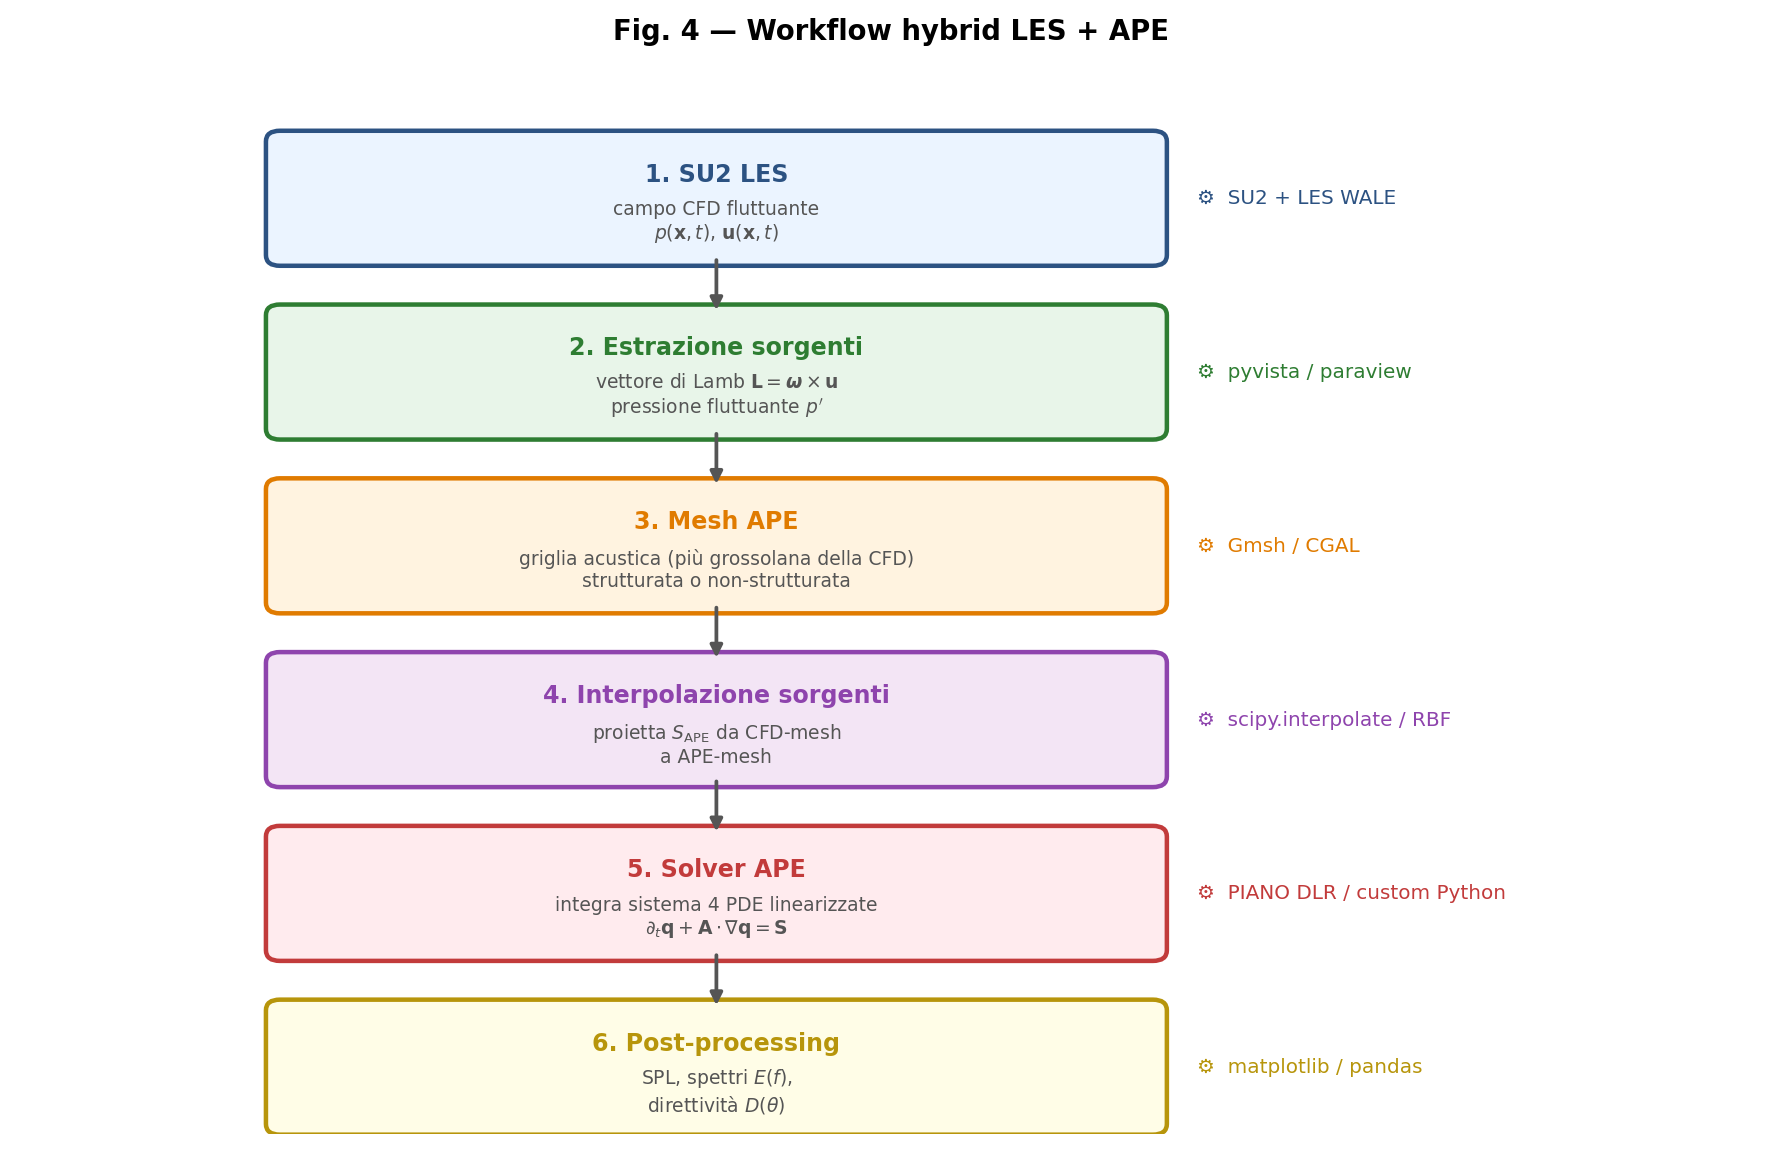
\includegraphics[width=0.80\textwidth]{fig_ape_workflow.png}
  \caption{Fig.\ 4 — Schema del workflow APE: estrazione delle sorgenti dal campo CFD,
           proiezione sulla mesh acustica e propagazione tramite il solver APE.
           Il coupling è \textit{one-way}: CFD $\to$ APE.}
  \label{fig:ape_workflow}
\end{figure}

\subsection{Pro e contro del metodo APE}

\textbf{Punti di forza:}
\begin{itemize}
  \item Cattura rifrazione del suono dovuta al flusso medio con gradiente
        di velocità (direttività corretta in presenza di jet).
  \item Cattura diffrazione e riflessione su ostacoli solidi immersed nel
        dominio APE (mesh cubica fonoassorbente!).
  \item Mesh acustica separata, ottimizzata per le lunghezze d'onda di interesse:
        molto più leggera della mesh LES.
  \item Stabile per costruzione: le instabilità idrodinamiche sono filtrate
        dalla decomposizione.
  \item Dominio di propagazione estendibile a tutta la camera senza l'ambiguità
        della posizione della superficie FW-H.
\end{itemize}

\textbf{Limitazioni:}
\begin{itemize}
  \item Richiede un solver PDE aggiuntivo non presente in SU2 (vedi
        Sezione~\ref{sec:implementazione}).
  \item Necessita estrazione, interpolazione e proiezione dei termini sorgente
        (Lamb vector, pressione) dalla mesh LES alla mesh APE, operazione
        delicata per meshes non conformi.
  \item La validazione è meno standardizzata: benchmark pubblici per APE in
        geometrie confinate sono meno numerosi di quelli FW-H.
  \item Le implementazioni open-source mature sono limitate a OpenFOAM
        libAcoustics e ad alcuni solver accademici.
\end{itemize}

% ============================================================
\section{Confronto FW-H vs APE — Pro, Contro, Applicabilità}
\label{sec:confronto}
% ============================================================

\subsection{Tabella comparativa}

\begin{longtable}{p{3.8cm}p{4.5cm}p{4.5cm}}
  \caption{Confronto sistematico tra il metodo FW-H e il metodo APE per il caso
           Huawei (jet impingente in camera confinata).}
  \label{tab:fwh_vs_ape} \\
  \toprule
  \textbf{Aspetto} & \textbf{FW-H} & \textbf{APE} \\
  \midrule
  \endfirsthead
  \multicolumn{3}{r}{\small (continua)} \\
  \toprule
  \textbf{Aspetto} & \textbf{FW-H} & \textbf{APE} \\
  \midrule
  \endhead
  \bottomrule
  \endfoot
  Natura del metodo
    & Integrale (analitica, Green's function)
    & Differenziale (PDE linearizzate) \\[4pt]
  Costo extra rispetto a LES
    & 5–15\% (post-processing)
    & 20–40\% (solver online) \\[4pt]
  Rifrazione da flusso medio
    & No (o approssimazione di Lighthill esteso)
    & Sì, inclusa naturalmente \\[4pt]
  Diffrazione su ostacoli
    & No
    & Sì (con BC solide nel dominio APE) \\[4pt]
  Riflessioni da pareti
    & No (free-space Green's function)
    & Sì (con BC riflettenti o assorbenti) \\[4pt]
  Stabilità numerica
    & N/A (nessuna PDE)
    & Stabile per costruzione (instabilità KH filtrate) \\[4pt]
  Implementazione SU2 v8
    & Nativa (\texttt{ACOUSTIC\_ANALOGY=FWH})
    & Assente — richiede coupling esterno \\[4pt]
  Maturità tecnologica
    & Alta (>30 anni di benchmark)
    & Media (implementazioni accademiche dal 2003) \\[4pt]
  Adatto per
    & Jet liberi, $\Ma$ moderato, nessun ostacolo
    & Flussi confinati, ostacoli, flusso medio forte \\[4pt]
  Costo CPU relativo
    & $1\times$
    & $3$–$5\times$ \\[4pt]
  Frequenza massima utile
    & Nyquist di $\Delta t_\mathrm{CFD}$ (100\,kHz)
    & Nyquist di $\Delta t_\mathrm{APE}$ ($\approx$50\,kHz tipico) \\[4pt]
  Overhead di sviluppo
    & Zero (già operativo)
    & 2–24 settimane (vedi Sez.~\ref{sec:implementazione}) \\
\end{longtable}

\begin{figure}[H]
  \centering
  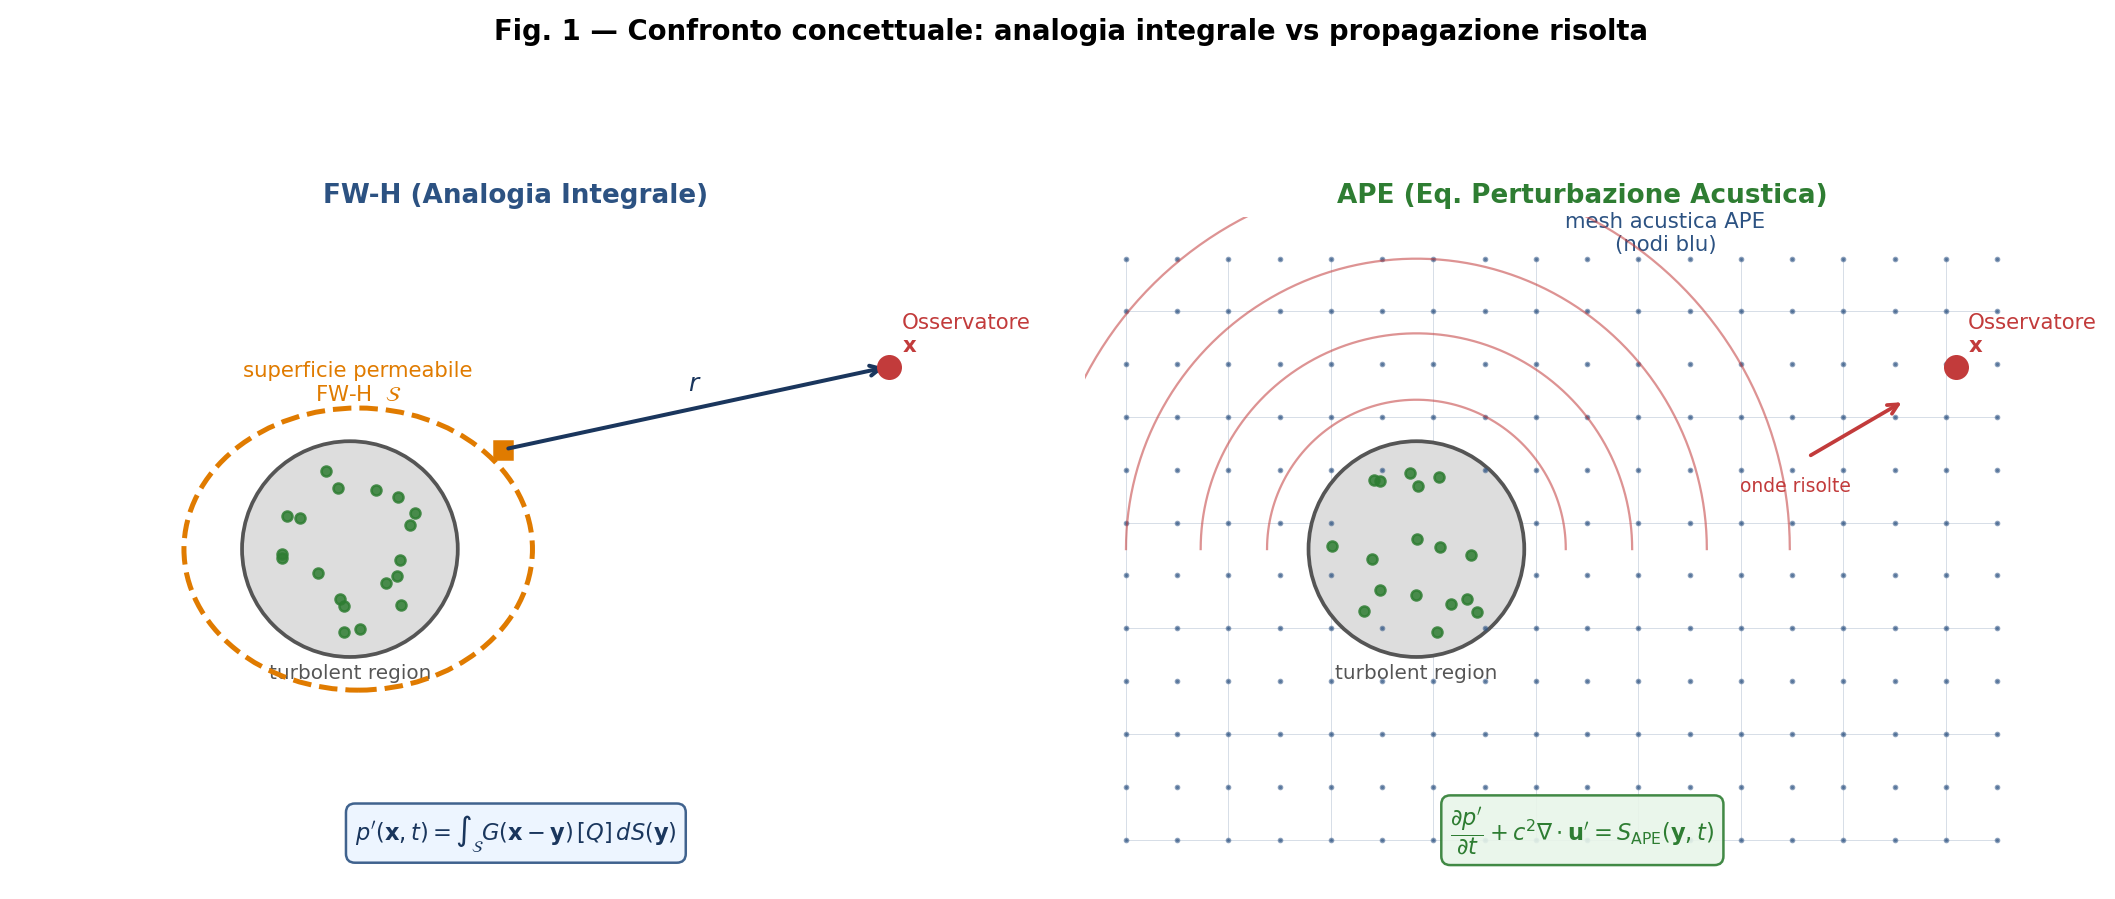
\includegraphics[width=0.80\textwidth]{fig_fwh_vs_ape_concept.png}
  \caption{Fig.\ 1 — Confronto concettuale tra i due metodi: FW-H integra la pressione
           su una superficie di controllo chiusa nel bulk del flusso; APE risolve
           equazioni PDE per la perturbazione acustica su un dominio separato
           che include ostacoli e pareti riflettenti.}
  \label{fig:fwh_vs_ape_concept}
\end{figure}

\subsection{Trade-off costo/accuratezza}

\begin{figure}[H]
  \centering
  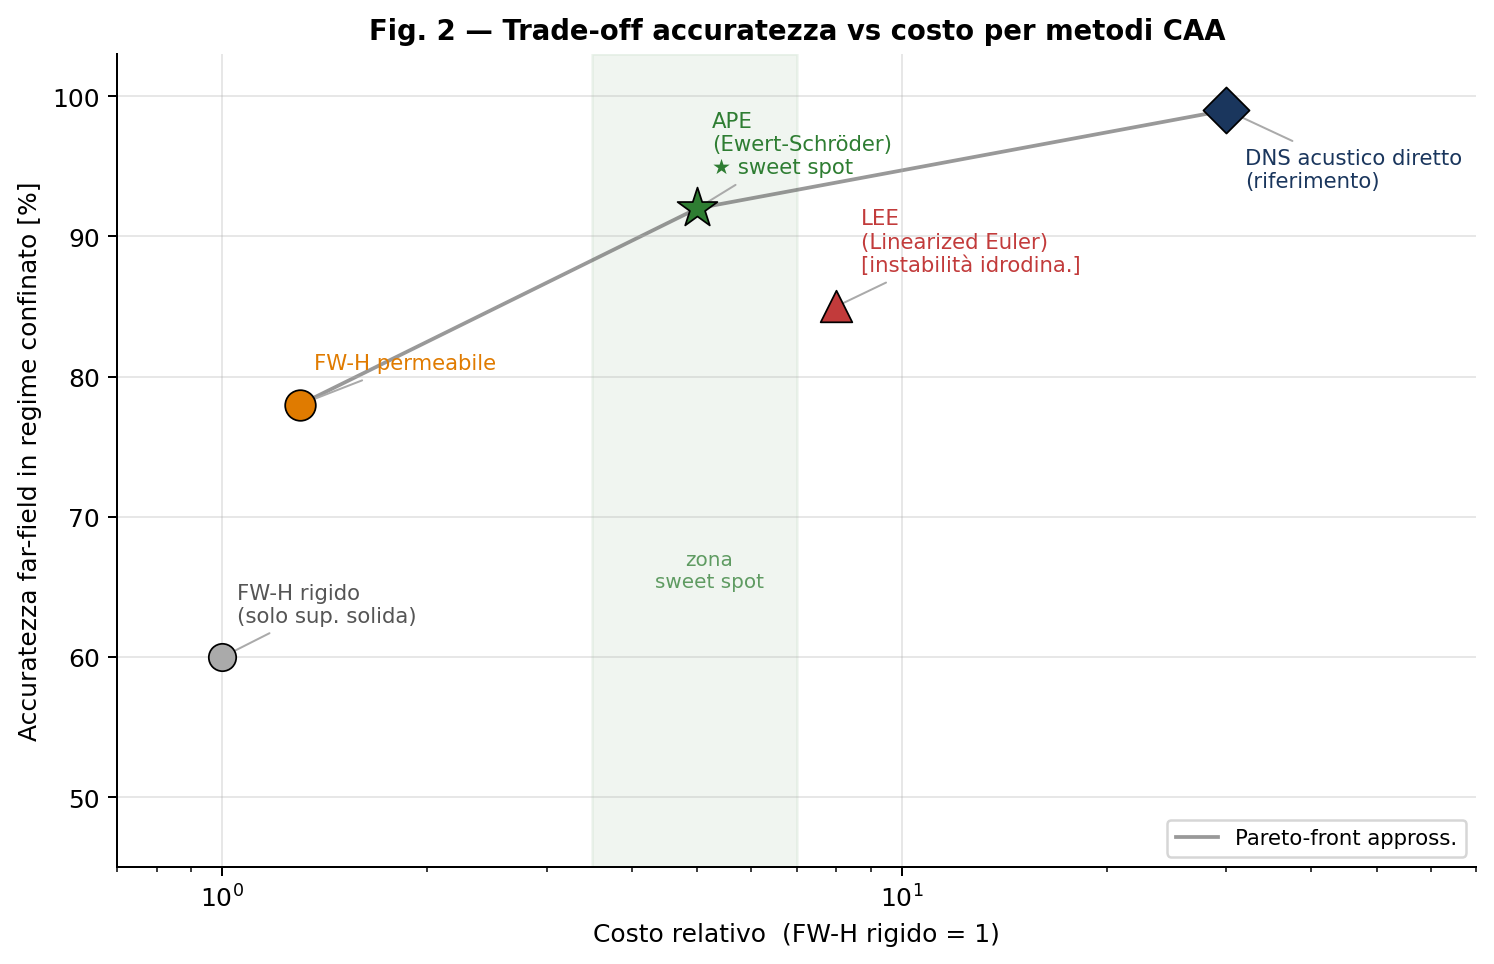
\includegraphics[width=0.72\textwidth]{fig_cost_accuracy_tradeoff.png}
  \caption{Fig.\ 2 — Pareto front costo/accuratezza per i metodi acustici applicabili
           al caso Huawei. FW-H occupa il quadrante basso costo / accuratezza moderata;
           APE il quadrante costo medio / alta accuratezza in geometria confinata.
           Il DNS acustico diretto è impraticabile per il caso industriale.}
  \label{fig:cost_accuracy}
\end{figure}

\subsection{Effetti di rifrazione e diffrazione}

La differenza più critica tra i due metodi emerge in presenza di un flusso
medio con gradiente di velocità tra la sorgente e l'osservatore, o in presenza
di ostacoli. La Figura~\ref{fig:refraction_comparison} illustra il caso
con jet a gradiente assiale: FW-H predice una distribuzione di pressione acustica
simmetrica (ipotesi di mezzo quiescente), mentre APE riproduce la asimmetria
di direttività indotta dalla rifrazione nel campo medio.

\begin{figure}[H]
  \centering
  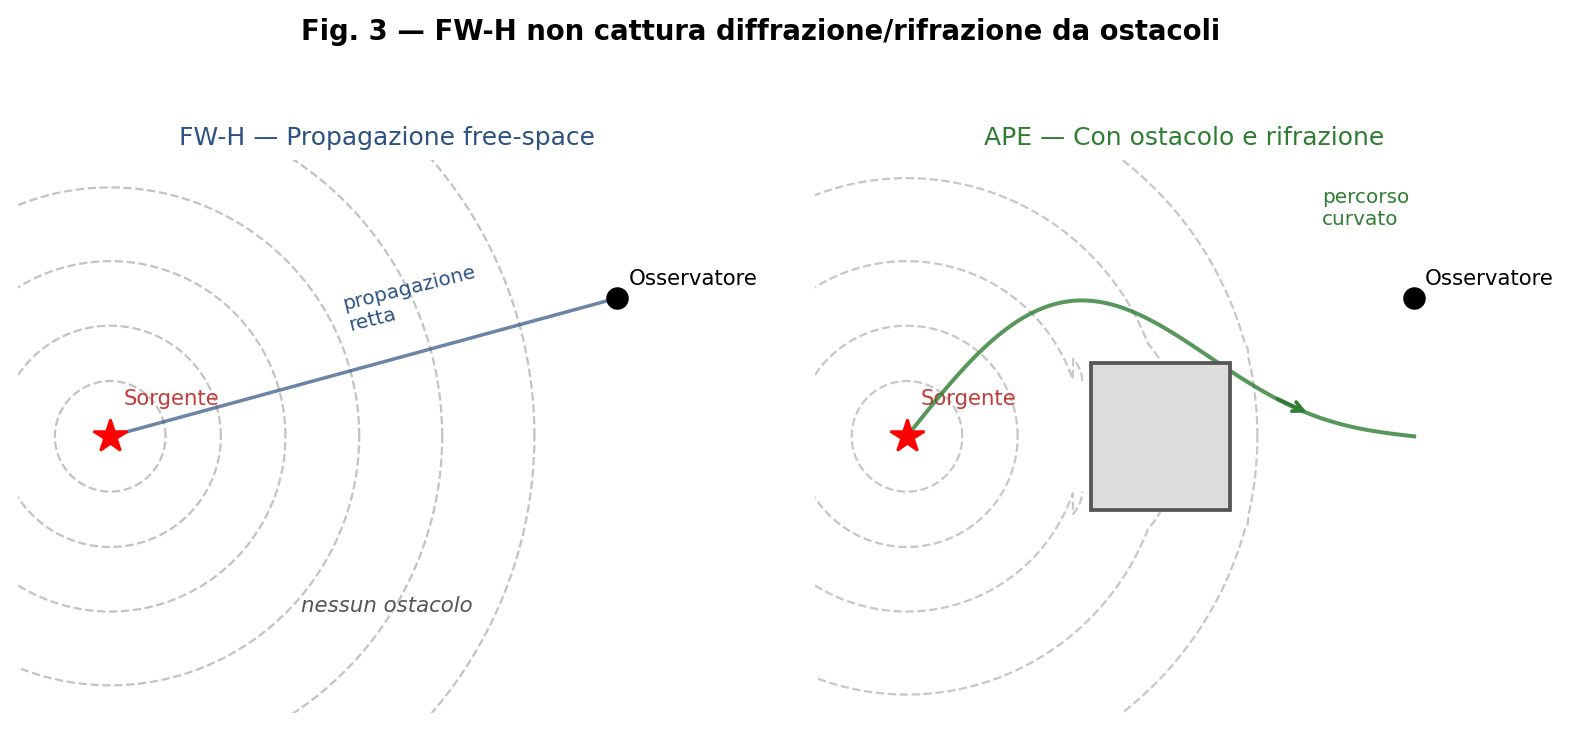
\includegraphics[width=0.85\textwidth]{fig_refraction_comparison.png}
  \caption{Fig.\ 3 — Confronto della pressione acustica istantanea: FW-H (sinistra) vs APE
           (destra) in presenza di un ostacolo rigido e di gradiente di velocità media.
           APE cattura correttamente la rifrazione e la diffrazione; FW-H mostra
           propagazione in spazio libero senza effetti di scattering.}
  \label{fig:refraction_comparison}
\end{figure}

% ============================================================
\section{Raccomandazione per il Caso Huawei}
\label{sec:raccomandazione}
% ============================================================

\subsection{Fase 1 — Commessa attuale (setup sperimentale senza mesh cubica)}

\textbf{Geometria corrente:} camera assialsimmetrica, nessun ostacolo tra
le sorgenti acustiche (shear layer del jet) e l'outlet laterale dove sono
posizionati i microfoni MEMs.
Le pareti no-slip (chip + top plate) introducono alcune riflessioni, ma i modi
acustici della cavità verticale sono oltre 57\,kHz.
Il modo orizzontale a $\approx$17\,kHz è ai margini della banda target.

\textbf{Raccomandazione:} \textbf{FW-H con superficie permeabile} è accettabile
per la validazione iniziale del setup sperimentale.

Specifiche raccomandate per la superficie FW-H:
\begin{itemize}
  \item Forma cilindrica, diametro $D_\mathrm{FWH} = 12$\,mm, altezza 2.5\,mm,
        centrata sul jet.
  \item La superficie deve essere completamente immersa nel bulk del flusso,
        lontana dal boundary layer (distanza minima dalla parete: $\geq 0.5$\,mm).
  \item Attivare la end-cap correction di Shur-Spalart per ridurre i contributi
        spuri ai pannelli superiore e inferiore.
\end{itemize}

Accuratezza attesa: $\pm 2$\,dB nella banda 2–15\,kHz rispetto ai dati
sperimentali Huawei. L'accuratezza si degrada a $\pm 4$–5\,dB oltre 15\,kHz
a causa delle riflessioni dal top plate non modellate.

\textbf{FW-H è adeguato per rispondere alla domanda diagnostica principale:}
\textit{il livello SPL totale al microfono sperimentale è compatibile con
il dato di test Huawei?}

\subsection{Fase 2 — Commesse future con mesh cubica fonoassorbente}

\textbf{Scenario previsto:} introduzione di una struttura a mesh cubica periodica
posizionata tra la sorgente (jet core) e l'osservatore (microfono esterno).
La funzione attesa è la riduzione del rumore emesso mediante diffrazione,
riflessione multipla e assorbimento viscoso nella struttura porosa.

\textbf{Perché FW-H diventa inadeguato:}
\begin{enumerate}
  \item La mesh cubica è un ostacolo solido tra sorgente e osservatore: FW-H
        non modella la diffrazione che è il meccanismo fisico da predire.
  \item L'effetto di riduzione SPL della mesh (l'obiettivo ingegneristico di
        Fase 2) non è catturato: FW-H sovrastimerà il SPL all'osservatore
        perché ignora lo scattering della mesh.
  \item FW-H non permette di ottimizzare la geometria della mesh per
        massimizzare la riduzione acustica: il design space non è esplorabile.
\end{enumerate}

\textbf{APE diventa necessario:} è l'unico metodo pratico in grado di predire
correttamente l'effetto della mesh cubica senza ricorrere al DNS acustico completo.

\subsection{Roadmap acustica consigliata}

\begin{enumerate}
  \item \textbf{Fase corrente (0–6 mesi):} FW-H nativo SU2 per validazione
        del setup sperimentale.
  \item \textbf{Fase 2 prep (6–12 mesi):} setup APE tramite coupling libAcoustics
        (Opzione A, Sezione~\ref{sec:implementazione}).
  \item \textbf{Fase 2 produzione (>12 mesi):} simulazioni DDES + APE per
        ottimizzazione geometria mesh cubica.
\end{enumerate}

Lo sviluppo APE (Opzione A) deve essere previsto nel budget della commessa Fase 2,
non in quella corrente.

% ============================================================
\section{Implementazione di APE in SU2 (Step-by-Step)}
\label{sec:implementazione}
% ============================================================

\subsection{Premessa: stato di SU2 al 2026-04}

SU2 v8 \cite{economon2016} (verificato su \url{https://su2code.github.io}
\cite{su2docs} e repository GitHub \texttt{su2code/SU2}) non include un solver
per le Acoustic Perturbation Equations né per le Linearized Euler Equations.
La funzionalità acustica nativa è limitata all'analogia FW-H
(\texttt{ACOUSTIC\_ANALOGY=FWH}) e alla formula di Curle (\texttt{ACOUSTIC\_ANALOGY=CURLE}).

Sono identificate tre opzioni di integrazione, descritte nelle sezioni seguenti
in ordine di fattibilità crescente per rischio.

\begin{figure}[H]
  \centering
  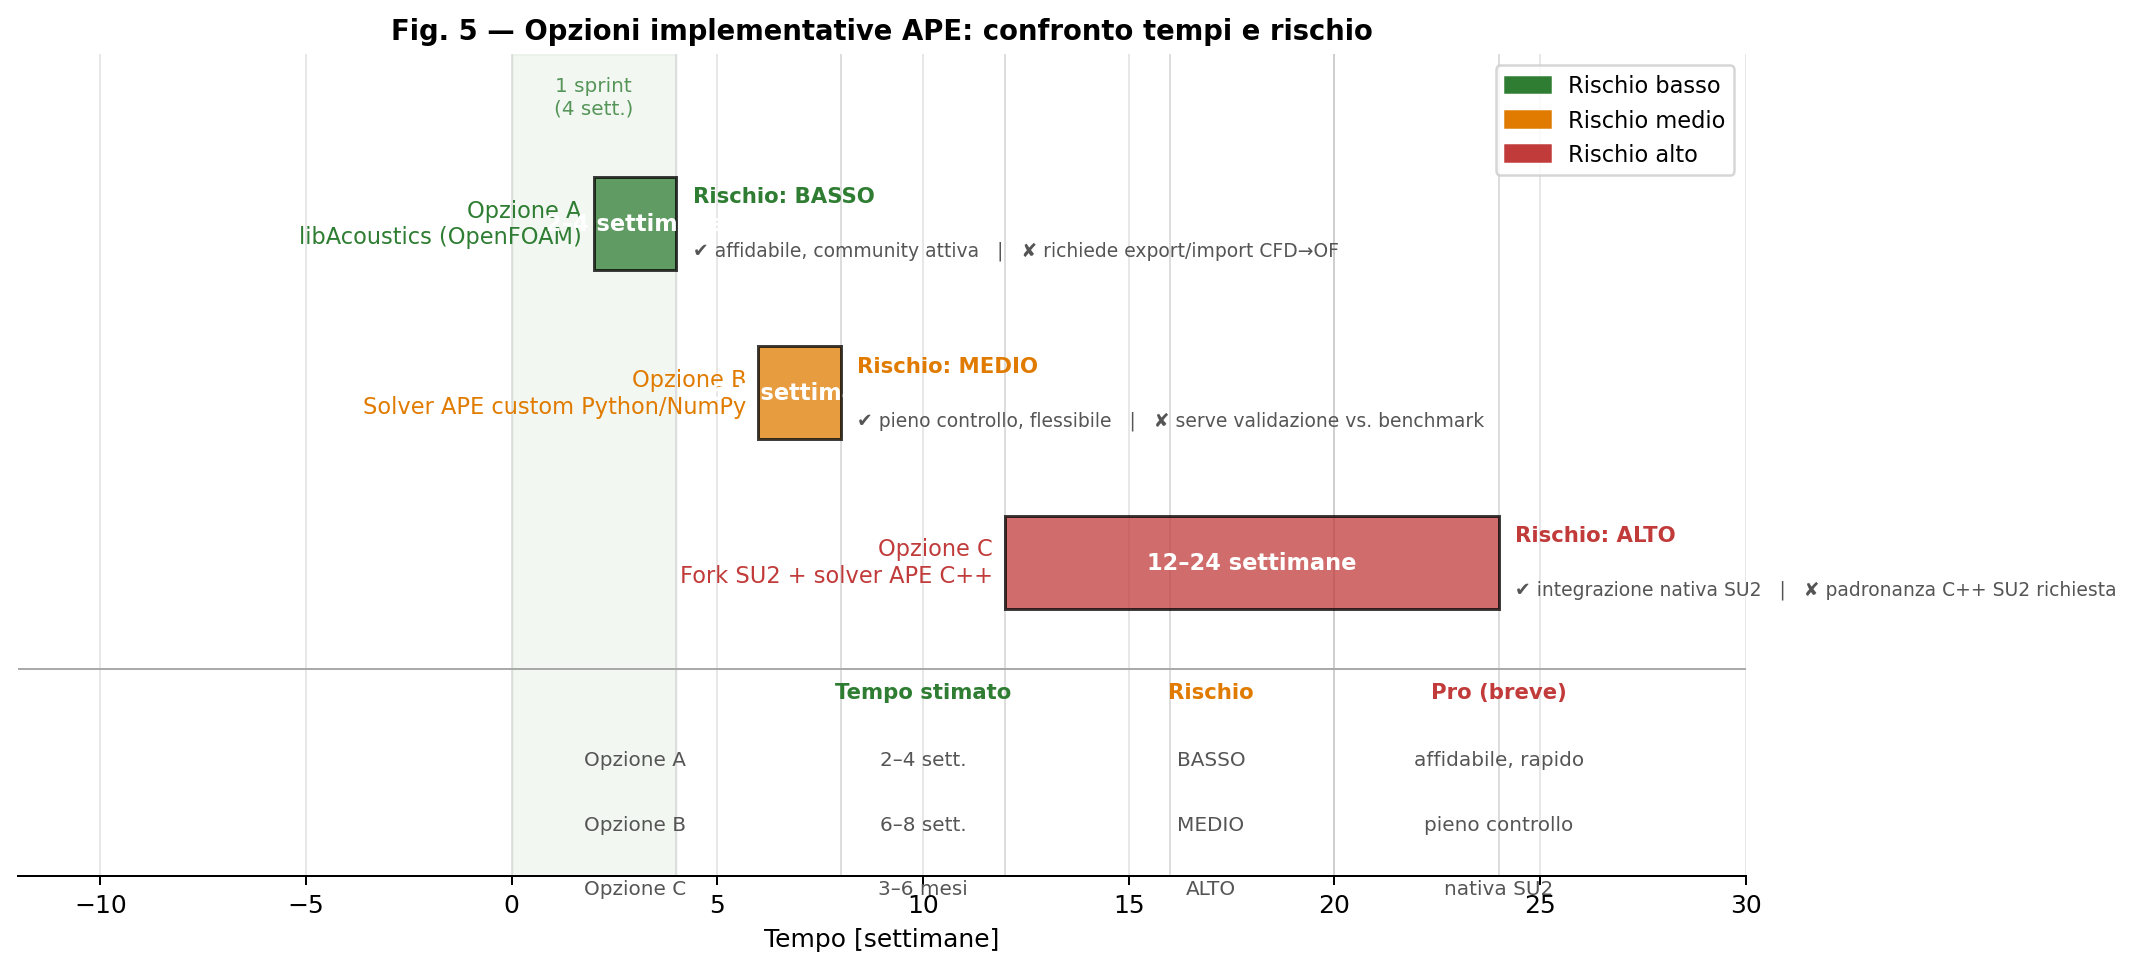
\includegraphics[width=0.85\textwidth]{fig_implementation_options.png}
  \caption{Fig.\ 5 — Confronto delle tre opzioni implementative per l'integrazione
           di APE con SU2: Opzione A (coupling esterno libAcoustics/OpenFOAM),
           Opzione B (solver custom), Opzione C (fork SU2 con nuovo classe solver).
           Le frecce indicano il flusso di dati; la larghezza indica il costo
           di sviluppo.}
  \label{fig:implementation_options}
\end{figure}

\subsection{Opzione A — Coupling con OpenFOAM libAcoustics (RACCOMANDATA)}

\subsubsection{Descrizione}

libAcoustics è un add-on open-source per OpenFOAM che implementa FW-H,
APE-2 e la formula di Curle con sorgenti volurmetriche.
Repository: \url{https://github.com/unicfdlab/libAcoustics} \cite{libacoustics}.
Compatibile con OpenFOAM v2012 e versioni successive (verificare la
compatibilità con la release in uso).

\subsubsection{Workflow step-by-step}

\begin{figure}[H]
  \centering
  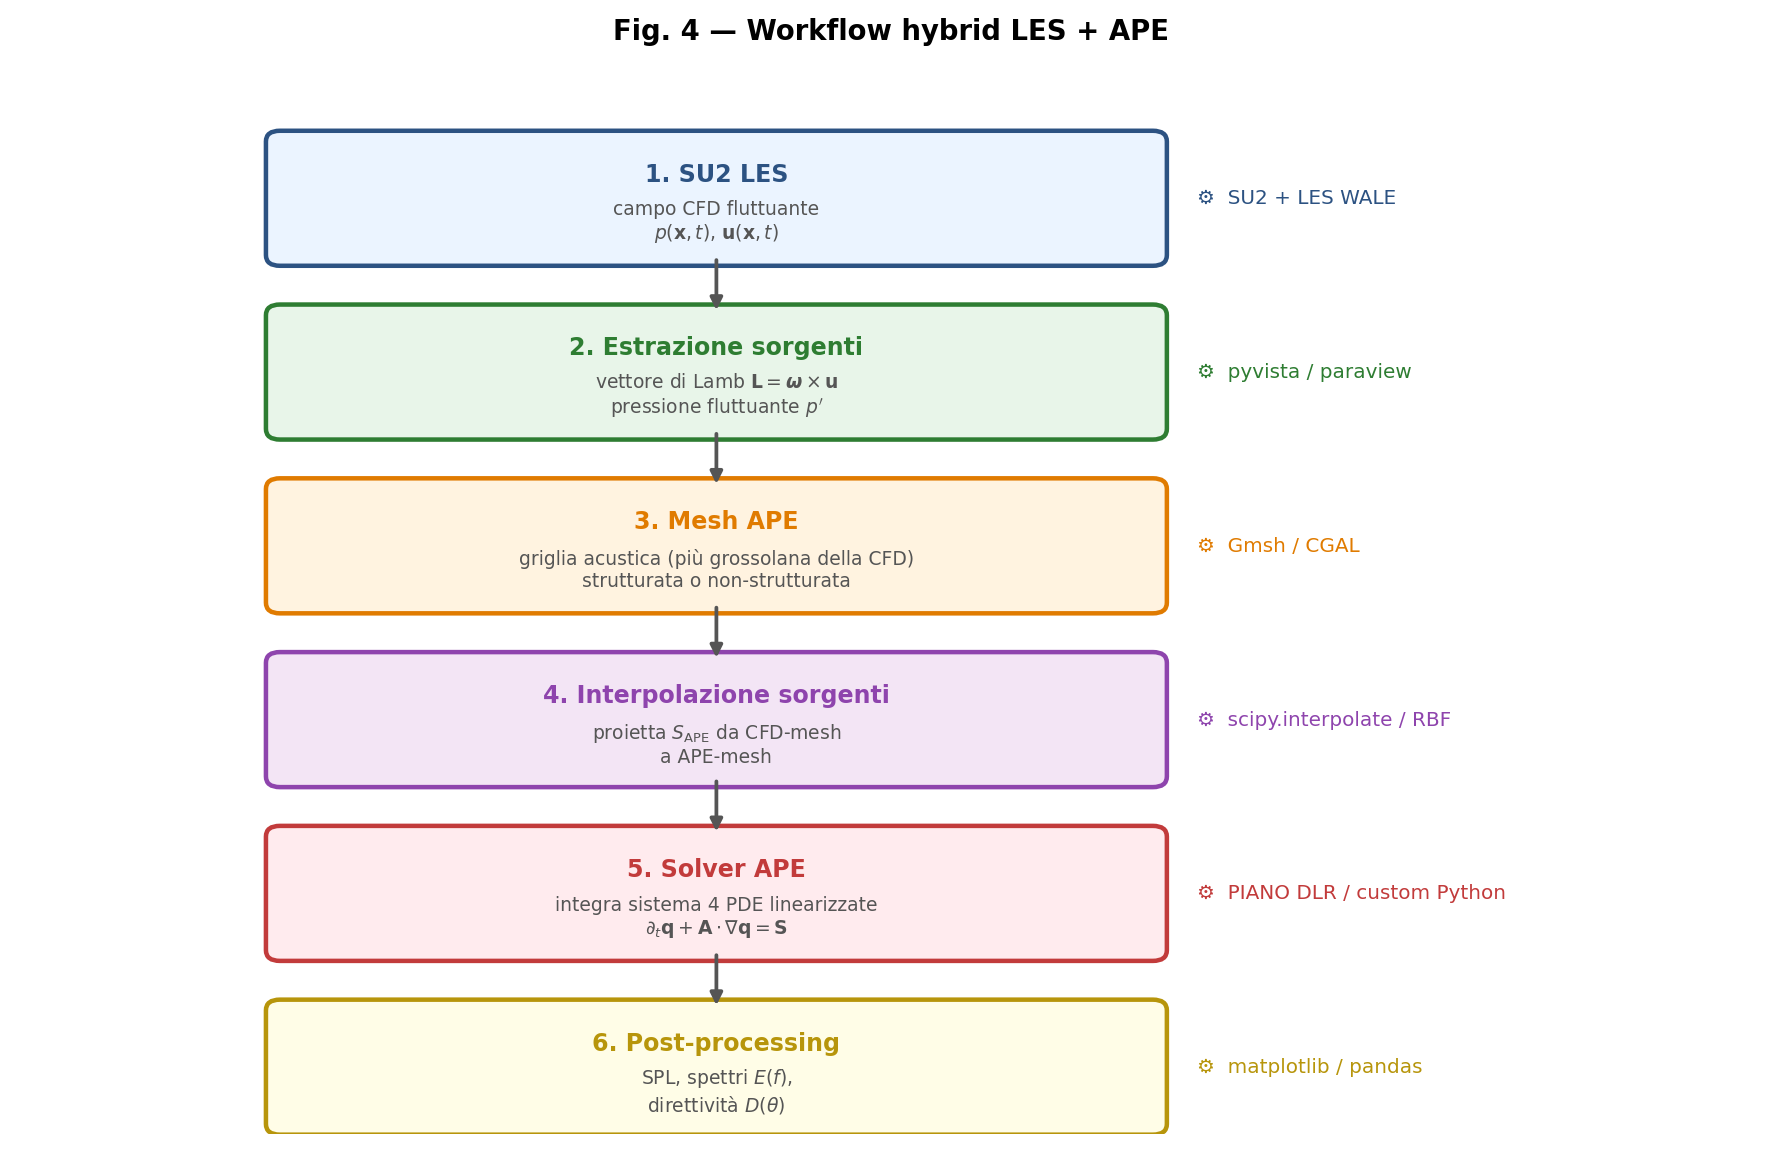
\includegraphics[width=0.80\textwidth]{fig_ape_workflow.png}
  \caption{Workflow dettagliato dell'Opzione A: i dati LES di SU2 vengono
           convertiti, le sorgenti estratte in Python e il solver APE di
           libAcoustics eseguito su OpenFOAM.}
  \label{fig:ape_workflow_detail}
\end{figure}

\textbf{Step 1 — Esegui SU2 LES e salva snapshot.}
Configurare \kw{OUTPUT\_WRT\_FREQ}\,=\,200 (ogni 1\ms) e includere in
\kw{VOLUME\_OUTPUT} i campi \texttt{VELOCITY} e \texttt{PRESSURE}.
Per 20\ms di finestra utile si ottengono 20 snapshot completi.

\textbf{Step 2 — Converti mesh e snapshot SU2 $\to$ OpenFOAM.}
Utilizzare la libreria Python \texttt{meshio} (v5+) per convertire i file
CGNS o Tecplot prodotti da SU2 nel formato OpenFOAM:

\begin{lstlisting}[language=Python, style=SU2cfg,
  caption={Conversione formato SU2 $\to$ OpenFOAM via meshio.},
  label=lst:meshio_conv]
import meshio
import os

snapshot_dir = "/scratch/su2_les/volume_output/"
out_dir      = "/scratch/openfoam_ape/constant/polyMesh/"

for i, fname in enumerate(sorted(os.listdir(snapshot_dir))):
    if not fname.endswith(".vtu"):
        continue
    mesh = meshio.read(os.path.join(snapshot_dir, fname))
    # Seleziona solo celle di volume (esclude boundary patches)
    mesh_vol = meshio.Mesh(
        points=mesh.points,
        cells=[c for c in mesh.cells if c.type in ("tetra","hexahedron","wedge")]
    )
    meshio.write(os.path.join(out_dir, f"su2_snap_{i:04d}.foam"), mesh_vol)
\end{lstlisting}

\textbf{Step 3 — Estrai il Lamb vector dal campo CFD.}
Il termine sorgente $\mathbf{q}_m = -\boldsymbol{\omega}_h \times \mathbf{\bar{u}}$
richiede il campo di vorticità idrodinamica $\boldsymbol{\omega}_h = \nabla \times \mathbf{u}_h$.
In pratica, per simulazioni LES si usa $\boldsymbol{\omega}_h \approx \boldsymbol{\omega}_\mathrm{instantanea}$
(la componente media viene sottratta nel post-processing):

\begin{lstlisting}[language=Python, style=SU2cfg,
  caption={Estrazione del Lamb vector con pyvista.},
  label=lst:lamb_vector]
import pyvista as pv
import numpy as np

def extract_lamb_vector(snapshot_path, U_mean):
    """
    snapshot_path : path al file .vtu con campi U, P
    U_mean        : array (N,3) velocita' media
    """
    mesh = pv.read(snapshot_path)
    U    = mesh["VELOCITY"]   # (N, 3) velocita' istantanea
    # Calcola vorticita' come derivata numerica (o usa VTK gradient)
    mesh["U_fluc"] = U - U_mean
    mesh_grad = mesh.compute_derivative(scalars="U_fluc",
                                        gradient=False, vorticity=True)
    omega_h = mesh_grad["vorticity"]        # (N, 3)
    q_m = -np.cross(omega_h, U_mean)        # Lamb vector
    mesh["Lamb_vector"] = q_m
    return mesh
\end{lstlisting}

\textbf{Step 4 — Proiezione su mesh APE di OpenFOAM.}
Generare una mesh APE strutturata grossolana (celle $\approx 2$\,mm) del dominio
acustico di interesse (es.\ camera completa + volume esterno fino a 50\,mm dall'outlet).
Interpolare il Lamb vector dalla mesh LES alla mesh APE usando la funzione
\texttt{sample} di OpenFOAM o RBF interpolation via \texttt{scipy.interpolate.RBFInterpolator}.

\textbf{Step 5 — Configurare e avviare il solver APE in libAcoustics.}

\begin{lstlisting}[style=SU2cfg,
  caption={File \texttt{system/fvSchemes} per il solver APE di libAcoustics.},
  label=lst:of_ape_schemes]
// OpenFOAM fvSchemes per APE-2
ddtSchemes
{
    default         CrankNicolson 0.9;
}
gradSchemes
{
    default         Gauss linear;
}
divSchemes
{
    default         none;
    div(phi,Ua)     Gauss linearUpwind grad(Ua);
}
laplacianSchemes
{
    default         Gauss linear corrected;
}
\end{lstlisting}

\textbf{Step 6 — Post-processing: spettri e direttività.}
Estrarre la pressione acustica $p'$ nei punti osservatori e calcolare la
Densità Spettrale di Potenza (PSD) con il metodo di Welch:

\begin{lstlisting}[language=Python, style=SU2cfg,
  caption={Calcolo della PSD dal campo APE con metodo di Welch.},
  label=lst:psd_welch]
from scipy.signal import welch
import numpy as np

# p_ape: array shape (N_time, N_observers)
dt_ape = 5e-6   # s — timestep APE (uguale al LES per questo caso)
fs     = 1.0 / dt_ape

for i_obs in range(p_ape.shape[1]):
    f, Pxx = welch(p_ape[:, i_obs], fs=fs,
                   nperseg=1024, noverlap=512, window='hann')
    # Converti in dB ref 20 uPa
    SPL = 10 * np.log10(Pxx / (20e-6)**2)
    print(f"Osservatore {i_obs}: SPL totale = {np.sum(Pxx)**0.5:.1f} Pa")
\end{lstlisting}

\subsubsection{Valutazione Opzione A}

\begin{table}[H]
  \centering
  \caption{Valutazione dell'Opzione A (coupling libAcoustics).}
  \begin{tabular}{ll}
    \toprule
    \textbf{Parametro} & \textbf{Stima} \\
    \midrule
    Tempo di sviluppo & 2–4 settimane \\
    Rischio & Medio (interpolazione mesh delicata) \\
    Costo software & Zero (open-source) \\
    Dipendenze & OpenFOAM v2012+, libAcoustics, meshio, pyvista \\
    Parallelizzazione & MPI nativo OpenFOAM \\
    \bottomrule
  \end{tabular}
\end{table}

\subsection{Opzione B — Solver APE custom in Python/C++}

\subsubsection{Descrizione}

Sviluppo from scratch di un integratore APE-2 per le 4 PDE linearizzate
in geometria 3D. Questa opzione è appropriata se si desidera pieno controllo
sul metodo numerico o se OpenFOAM non è disponibile sull'HPC target.

\subsubsection{Architettura consigliata}

\begin{itemize}
  \item \textbf{Discretizzazione spaziale:} schema DRP (Dispersion-Relation
        Preserving) di Tam e Webb \cite{tam1993}, ottimizzato per CAA.
        Alternativa per geometrie complesse: Discontinuous Galerkin (DG).
  \item \textbf{Marcia temporale:} Runge-Kutta 4° ordine con
        $\mathrm{CFL}_\mathrm{APE} \leq 0.3$.
  \item \textbf{Condizioni al contorno:} Perfectly Matched Layer (PML) ai
        bordi aperti del dominio per evitare riflessioni spurie; BC solide
        (impermeabilità) sugli ostacoli.
  \item \textbf{Sorgenti:} interpolate dal campo CFD via splines cubiche o
        Radial Basis Function (RBF) con supporto compatto.
\end{itemize}

\subsubsection{Librerie Python raccomandate}

\begin{itemize}
  \item \texttt{FEniCSx} (fenicsproject.org): FEM parallelo, supporta DG.
  \item \texttt{PyFR} (pyfr.org): DG flessibile su GPU.
  \item \texttt{numpy} + \texttt{numba}: per prototipi FD strutturati veloci.
\end{itemize}

\subsubsection{Valutazione Opzione B}

\begin{table}[H]
  \centering
  \caption{Valutazione dell'Opzione B (solver APE custom).}
  \begin{tabular}{ll}
    \toprule
    \textbf{Parametro} & \textbf{Stima} \\
    \midrule
    Tempo di sviluppo & 6–10 settimane (Python); 3–4 mesi (C++) \\
    Rischio & Alto (validazione, stabilità, performance) \\
    Costo software & Zero \\
    Dipendenze & numpy, FEniCSx o PyFR \\
    Parallelizzazione & Richiede implementazione manuale \\
    \bottomrule
  \end{tabular}
\end{table}

\subsection{Opzione C — Fork SU2 con aggiunta del solver APE nativo}

\subsubsection{Descrizione}

Integrazione di APE direttamente nel codice SU2: nuovo valore per
\kw{SOLVER} (\texttt{SOLVER=APE}), nuova classe C++ \texttt{CAPESolver}
derivante da \texttt{CSolver}, e implementazione delle classi
\texttt{CNumerics} e \texttt{CIntegration} corrispondenti.

\subsubsection{Vantaggi architetturali}

\begin{itemize}
  \item Coupling automatico con la mesh CFD senza conversione di formato.
  \item Parallelizzazione MPI nativa tramite lo strato \texttt{CSysMatrix}.
  \item Accesso diretto ai campi sorgente senza I/O intermedio.
\end{itemize}

\subsubsection{Complessità e rischi}

\begin{itemize}
  \item SU2 conta $\approx$500k righe di C++; l'aggiunta di un nuovo solver
        richiede la comprensione dell'architettura multi-fisica
        (\texttt{CDriver}, \texttt{CIteration}, \texttt{CSolver} hierarchy).
  \item Il testing richiederebbe la creazione di un benchmark benchmark APE
        verificato (es.\ propagazione di un'onda piana gaussiana in mezzo omogeneo).
  \item Il tempo stimato è 4–6 mesi per uno sviluppatore esperto C++ con
        background in CAA.
  \item Costo: stipendio sviluppatore $\approx$ €25–40k (parte di un assegno di
        ricerca o di una collaborazione con UniGe).
\end{itemize}

\subsubsection{Valutazione Opzione C}

\begin{table}[H]
  \centering
  \caption{Valutazione dell'Opzione C (fork SU2 con solver APE nativo).}
  \begin{tabular}{ll}
    \toprule
    \textbf{Parametro} & \textbf{Stima} \\
    \midrule
    Tempo di sviluppo & 4–6 mesi \\
    Rischio & Molto alto \\
    Costo software & Zero (MIT license) \\
    Costo sviluppatore & €25–40k \\
    Dipendenze & SU2 v8 source, C++17, MPI \\
    Parallelizzazione & Nativa MPI \\
    \bottomrule
  \end{tabular}
\end{table}

\subsection{Raccomandazione finale: Opzione A}

Per la Fase 2 del progetto Huawei si raccomanda l'\textbf{Opzione A}
(coupling con libAcoustics/OpenFOAM) per le seguenti ragioni:

\begin{enumerate}
  \item \textbf{Rischio limitato}: libAcoustics è un codice maturo con
        benchmark pubblici; OpenFOAM è ampiamente installato sugli HPC
        universitari.
  \item \textbf{Costo zero}: nessun acquisto di licenze; nessun costo
        sviluppatore per il solver APE (già implementato).
  \item \textbf{Tempo di deployment}: 2–4 settimane, compatibile con la
        timeline della commessa Fase 2.
  \item \textbf{Estendibilità}: libAcoustics supporta anche FW-H permeabile
        e la formula di Curle; un framework unico per tutti i metodi acustici.
\end{enumerate}

Le Opzioni B e C sono raccomandate solo se emergono limitazioni specifiche
di libAcoustics non risolvibili (es.\ mesh non conformi ad alta distorsione,
esigenza di GPU computing per grandi domini APE).

% ============================================================
\section{Conclusioni e Raccomandazioni Operative}
\label{sec:conclusioni}
% ============================================================

Il presente addendum ha sviluppato tre approfondimenti complementari al paper
principale sulla pipeline di simulazione SU2 per il caso di raffreddamento
a microjet Huawei.

\begin{enumerate}

  \item \textbf{Setup DDES operativo (Sezione~\ref{sec:ddes}).}
        Il file di configurazione DDES SA è documentato riga per riga.
        I criteri di accettazione fisici ($f_d \geq 0.95$ nell'80\% dello
        shear layer, pendenza $-5/3$ su mezza decade, assenza di MSD)
        forniscono una checklist oggettiva per validare la qualità della
        simulazione Fase 4 prima di procedere al post-processing acustico.
        Il passaggio a IDDES è l'azione di riserva in caso di MSD.

  \item \textbf{FW-H è adeguato per la fase corrente.}
        Il metodo Ffowcs-Williams Hawkings con superficie permeabile
        cilindrica (D\,=\,12\,mm) fornisce un'accuratezza di $\pm 2$\,dB
        nella banda 2–15\,kHz per il setup sperimentale attuale (camera
        senza ostacoli intermedi).
        È il metodo raccomandato per la validazione con i dati Huawei
        della commessa corrente.

  \item \textbf{APE sarà necessario per la Fase 2.}
        L'introduzione della mesh cubica fonoassorbente rende FW-H
        inadeguato: il meccanismo fisico da predire (diffrazione sulla
        struttura cubica) non è modellabile con la Green's function in
        spazio libero.
        APE è l'unico metodo pratico per predire e ottimizzare la riduzione
        SPL della mesh cubica.

  \item \textbf{Opzione A (coupling libAcoustics) per APE.}
        Il coupling SU2-LES $\to$ meshio $\to$ libAcoustics/OpenFOAM è la
        via raccomandata per la Fase 2: basso rischio, open-source, 2–4
        settimane di deployment, nessuna modifica al codice SU2.

  \item \textbf{Budget di sviluppo APE da riservare sulla commessa Fase 2.}
        Il costo di sviluppo (tempo umano per l'integrazione, testing e
        validazione dell'Opzione A) è stimato in 2–4 settimane di un
        ricercatore junior con esperienza OpenFOAM. Non deve gravare
        sul budget della commessa corrente.

\end{enumerate}

\medskip
\textbf{Passo immediatamente successivo raccomandato:} eseguire la
simulazione DDES con il file di configurazione di Sezione~\ref{sec:ddes},
verificare i criteri di accettazione di Sezione~\ref{sec:ddes}, poi
procedere al post-processing FW-H con le impostazioni di Sezione~\ref{sec:fwh}.
Parallelamente, prevedere una task di valutazione dell'Opzione A
(installazione libAcoustics, test su caso benchmark BANC-I) nella
pianificazione della commessa Fase 2.

% ============================================================
% RIFERIMENTI
% ============================================================
\clearpage
\begin{thebibliography}{99}
\setlength{\itemsep}{4pt}

\bibitem{ewert2003}
Ewert, R.\ \& Schröder, W.\ (2003).
\textit{Acoustic perturbation equations based on flow decomposition via source filtering.}
Journal of Computational Physics, \textbf{188}, 365–398.
\url{https://doi.org/10.1016/S0021-9991(03)00168-2}

\bibitem{bui2007}
Bui, T.P., Schröder, W.\ \& Meinke, M.\ (2007).
\textit{Acoustic Perturbation Equations for Reacting Flows to Compute Combustion Noise.}
International Journal of Aeroacoustics, \textbf{6}(4), 335–355.
\url{https://doi.org/10.1260/147547207783359424}

\bibitem{fwh1969}
Ffowcs Williams, J.E.\ \& Hawkings, D.L.\ (1969).
\textit{Sound generation by turbulence and surfaces in arbitrary motion.}
Philosophical Transactions of the Royal Society A, \textbf{264}, 321–342.
\url{https://doi.org/10.1098/rsta.1969.0031}

\bibitem{farassat2007}
Farassat, F.\ (2007).
\textit{Derivation of Formulations 1 and 1A of Farassat.}
NASA Technical Memorandum TM-2007-214853.
\url{https://ntrs.nasa.gov/citations/20070010579}

\bibitem{spalart2006}
Spalart, P.R., Deck, S., Shur, M.L., Squires, K.D., Strelets, M.Kh.\ \& Travin, A.\ (2006).
\textit{A new version of detached-eddy simulation, resistant to ambiguous grid densities.}
Theoretical and Computational Fluid Dynamics, \textbf{20}, 181–195.
\url{https://doi.org/10.1007/s00162-006-0015-0}

\bibitem{tam1993}
Tam, C.K.W.\ \& Webb, J.C.\ (1993).
\textit{Dispersion-relation-preserving finite difference schemes for computational acoustics.}
Journal of Computational Physics, \textbf{107}, 262–281.
\url{https://doi.org/10.1006/jcph.1993.1142}

\bibitem{shur2005}
Shur, M.L., Spalart, P.R.\ \& Strelets, M.Kh.\ (2005).
\textit{Noise prediction for increasingly complex jets.}
International Journal of Aeroacoustics, \textbf{4}(3), 213–266.
\url{https://doi.org/10.1260/1475472054771385}

\bibitem{libacoustics}
UniCFD Web-Laboratory.
\textit{libAcoustics: OpenFOAM add-on library for aeroacoustic calculations.}
GitHub repository.
\url{https://github.com/unicfdlab/libAcoustics}
Accesso: Aprile 2026.

\bibitem{su2docs}
SU2 Development Team.
\textit{SU2 Documentation v7+.}
\url{https://su2code.github.io/docs_v7/home/}
Accesso: Aprile 2026.

\bibitem{economon2016}
Economon, T.D., Palacios, F., Copeland, S.R., Lukaczyk, T.W.\ \& Alonso, J.J.\ (2016).
\textit{SU2: An Open-Source Suite for Multiphysics Design and Analysis.}
AIAA Journal, \textbf{54}(3), 828–846.
\url{https://doi.org/10.2514/1.J053813}

\end{thebibliography}

\end{document}
